\documentclass[10pt,twocolumn,a4paper]{article}
\usepackage[a4paper,margin=1.4cm,top=1.2cm,bottom=1.4cm,columnsep=0.6cm]{geometry}
\usepackage[T1]{fontenc}
\usepackage[scaled=0.93]{helvet}
\renewcommand{\familydefault}{\sfdefault}
\usepackage{amsmath,amssymb,graphicx,booktabs,tabularx,xcolor,enumitem,titlesec,tikz}
\usetikzlibrary{arrows.meta}
\usepackage[hidelinks]{hyperref}
\usepackage[font=small,labelfont=bf,skip=3pt]{caption}
\graphicspath{{../figures/}}

\definecolor{accent}{HTML}{4B3FB5}
\definecolor{soft}{HTML}{EEECFA}
\titleformat{\section}{\large\bfseries\color{accent}}{\thesection.}{0.4em}{}
\titlespacing*{\section}{0pt}{6pt}{2pt}
\setlist{nosep,leftmargin=1.1em}
\setlength{\parindent}{0pt}
\setlength{\parskip}{3pt}
\setlength{\textfloatsep}{7pt}
\setlength{\floatsep}{6pt}
\setlength{\dbltextfloatsep}{7pt}
\raggedbottom
\newcommand{\term}[1]{\textbf{#1}}
\newcommand{\stat}[2]{\parbox[t]{0.23\textwidth}{\centering{\Huge\bfseries\color{accent}#1}\\[2pt]\small #2}}

\begin{document}

\twocolumn[{%
\begin{center}
{\LARGE\bfseries\color{accent} SafeLane-RL: Teaching a Car to Drive and Merge Safely with Reinforcement Learning}\\[5pt]
{\large Gokul Bansal (B24CM1025) \quad$\cdot$\quad Likhita (B24CM1043)}\\[2pt]
AI Course, Assignment 2 (Real-Life Use Cases of RL), IIT Jodhpur\\[1pt]
GitHub: \url{https://github.com/Osptium-Invincible/safelane-rl}
\end{center}
\vspace{1pt}
\noindent\colorbox{soft}{\parbox{\dimexpr\textwidth-2\fboxsep}{\centering\vspace{4pt}
\stat{0\%}{crashes on the official highway test\\(150 episodes)}\hfill
\stat{97--99\%}{successful merges from the on-ramp\\(plain PPO: 51\%)}\hfill
\stat{94\%}{merges in \textbf{2$\times$} the traffic it trained on\\(rule-based driver: 72\%)}\hfill
\stat{10.5\,h}{CPU-hours of training for all 61 runs, on one laptop (no GPU)}\vspace{4pt}}}
\vspace{7pt}
}]

\section{The problem}
Changing lanes and merging from an on-ramp are among the riskiest highway manoeuvres: the driver must judge gaps in moving traffic,
adjust speed, and commit before the ramp ends. Hand-written rule-based drivers are predictable but rigid, and in heavy traffic
they either refuse to merge or merge unsafely. We train a car to make these \term{tactical decisions} (which lane, faster or slower)
\emph{purely by trial and error} with reinforcement learning (RL); simple controllers do the steering and throttle, as in real
self-driving cars. Our main idea: treat safety as a \term{budget} the agent must respect, not as one more term in the reward.
We call the agent \term{SafeLane}.

\section{Simulator and scenarios}
We use \term{highway-env} 1.12.1, the standard RL simulator for highway driving. The other cars react to us: \term{IDM} sets their
speed (keep a safe gap to the car ahead) and \term{MOBIL} decides their lane changes. We made traffic more varied: each car has its own
reaction gap (0.5--2.5\,s) and politeness, and drivers can be normal, aggressive or cautious.
\begin{itemize}
\item \term{Highway:} train on 3 lanes with 20 cars; test on the official \texttt{highway-v0} (4 lanes, 50 cars, 40\,s).
\item \term{RampMerge (built by us):} our car starts on the on-ramp and must merge within 80\,m before the ramp ends at a barrier
(Fig.~\ref{fig:frames}). \emph{Success} = merged and passed the merge zone without crashing. (highway-env's own merge scenario puts
our car on the main road, so it cannot measure this.) Along the way we found and fixed a highway-env bug: a car on the ramp
``saw'' main-road cars as if they were in front of it.
\end{itemize}


\begin{figure}[t]\centering
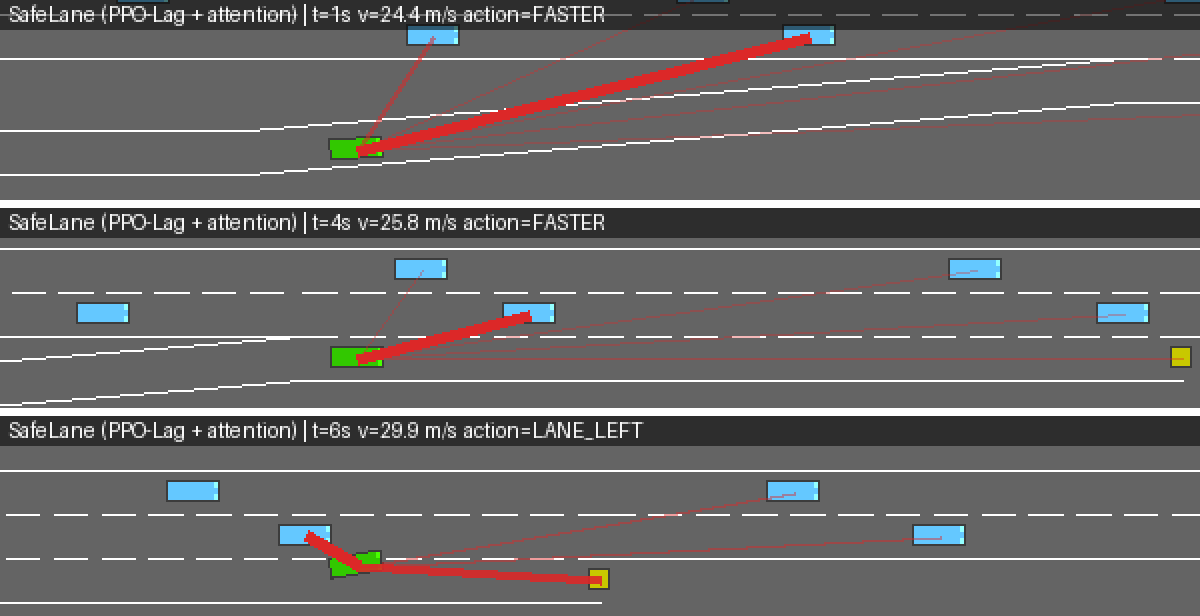
\includegraphics[width=\columnwidth]{ramp_frames.png}
\caption{SafeLane merging (frames from our GIF). Green = our car, blue = traffic, yellow = end-of-ramp barrier; red lines =
where the attention network is ``looking''. Top: on the ramp, speeding up. Middle: barrier ahead, choosing a gap. Bottom: moving left into the gap.}
\label{fig:frames}
\end{figure}

\begin{figure*}[t]\centering
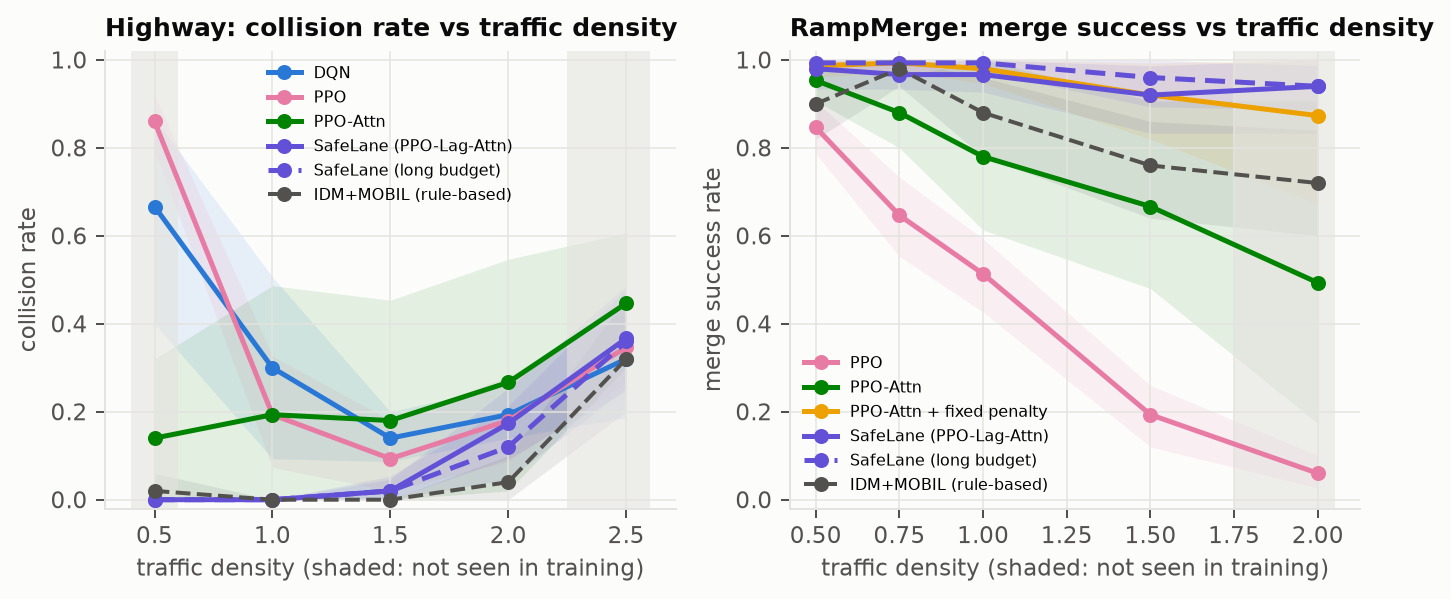
\includegraphics[width=0.74\textwidth]{density_sweep.png}
\caption{Lighter and heavier traffic than in training (grey shading = never seen in training). Left: highway crash rate (lower is better).
Right: merge success (higher is better). SafeLane is purple.}
\label{fig:density}
\end{figure*}

\section{RL formulation}
One \term{step} = one driving decision, made once per second. One \term{episode} = one drive; it ends early on a crash.

\smallskip
\renewcommand{\arraystretch}{1.2}
\noindent\begin{tabularx}{\columnwidth}{@{}>{\raggedright\bfseries\leavevmode\color{accent}}p{1.25cm}X@{}}
\toprule
State $S$ & A table of nearby cars: one row per car (ours first, then the nearest), with position and speed \emph{relative to us},
scaled to $[-1,1]$. Plain networks: 5 cars $\times$ 5 numbers $=25$. Attention network: 15 cars $\times$ 7 numbers $=105$.
Only cars within 200\,m are visible.\\
Action $A$ & 5 discrete choices: \textsc{lane-left}, \textsc{idle}, \textsc{lane-right}, \textsc{faster}, \textsc{slower}
(target speeds 10--30\,m/s).\\
Reward $R$ & \emph{Highway:} $r=\text{scale}_{[0,1]}(-1\cdot\text{crash}+0.1\cdot\text{lane}+0.4\cdot\text{speed})$; ``speed'' maps
20--30\,m/s to 0--1, ``lane'' rewards keeping right.\newline
\emph{Ramp:} $r=-1\cdot\text{crash}+0.2\cdot\text{speed}+1\cdot\text{merged}$.\newline
A crash also ends the episode, losing all future reward.\\
Cost $c$ & $c=[\text{TTC}<2\,\text{s}]+[\text{headway}<1\,\text{s}]+10\cdot[\text{crash}]$, where TTC (time-to-collision) = gap $\div$
closing speed and headway = gap $\div$ our speed. \textbf{Budget:} average episode cost $\le d=2$.\\
Discount & $\gamma=0.9$: the agent plans about 10\,s ahead.\\
\bottomrule
\end{tabularx}

\section{Our agent: SafeLane}
SafeLane = three ingredients (Fig.~\ref{fig:loop}):
\begin{enumerate}
\item \term{PPO}: a policy-gradient algorithm that directly learns how likely each action should be, improving it in small, safe steps
(8 simulators in parallel).
\item \term{Attention network} (written by us): every car is encoded by the same small network, and our car ``asks'' which cars matter
right now. It handles any number of cars and its weights can be drawn (red lines in Fig.~\ref{fig:frames}). 46.7k parameters vs 146k for a plain network.
\item \term{Safety budget} (PPO-Lagrangian, a \emph{constrained MDP}): maximise reward \emph{such that} average episode cost $\le d$.
The agent maximises $r-\lambda c$, and the safety weight $\lambda$ is \emph{learned}: over budget $\Rightarrow$ $\lambda$ goes up (safety
matters more); under budget $\Rightarrow$ $\lambda$ goes down (speed matters again). A PID controller updates $\lambda$ every 1{,}024 steps. In training, the episode cost started at 10--13 and was pushed down to the budget of 2; $\lambda$ rose while the agent was unsafe, then fell.
\end{enumerate}
\term{Why not just a big crash penalty?} Its right size is unknown (too small: crashes; too large: the car crawls) and must be
re-tuned per task. A budget is set once, in understandable units.

\begin{figure}[t]\centering
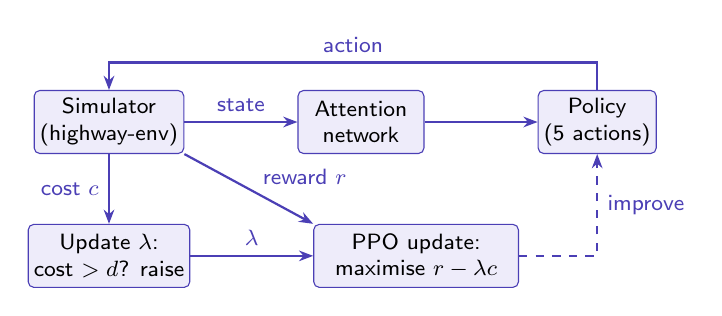
\begin{tikzpicture}[font=\footnotesize,
  box/.style={draw=accent, fill=soft, rounded corners=2pt, align=center, minimum height=8mm, inner sep=2pt},
  ar/.style={-{Stealth[length=1.8mm]}, thick, accent}]
\node[box, minimum width=1.9cm] (sim) at (0,0) {Simulator\\(highway-env)};
\node[box, minimum width=1.6cm] (att) at (3.2,0) {Attention\\network};
\node[box, minimum width=1.5cm] (pol) at (6.2,0) {Policy\\(5 actions)};
\node[box, minimum width=1.9cm] (lam) at (0,-1.7) {Update $\lambda$:\\cost $>d$? raise};
\node[box, minimum width=2.6cm] (ppo) at (3.9,-1.7) {PPO update:\\maximise $r-\lambda c$};
\draw[ar] (sim) -- node[above]{state} (att);
\draw[ar] (att) -- (pol);
\draw[ar] (pol.north) -- ++(0,0.35) -| node[pos=0.25,above]{action} (sim.north);
\draw[ar] (sim) -- node[left]{cost $c$} (lam);
\draw[ar] (sim.south east) -- node[pos=0.55,above right=-1pt]{reward $r$} (ppo.north west);
\draw[ar] (lam) -- node[above]{$\lambda$} (ppo);
\draw[ar, dashed] (ppo.east) -| node[pos=0.75,right]{improve} (pol.south);
\end{tikzpicture}
\caption{How SafeLane learns.}
\label{fig:loop}
\end{figure}

\section{What we compared, and how}
\begin{itemize}
\item \term{Baselines:} random; constant speed; a \term{rule-based driver} (IDM+MOBIL; on the ramp it matches speed and merges into gaps $\ge$ 0.8\,s).
\item \term{Value-based RL:} DQN; our D3QN (Double + Dueling + 3-step DQN); QR-DQN.
\item \term{PPO family:} PPO; PPO + attention; the same with a \emph{fixed} penalty ($\lambda=0.1$); MaskablePPO, where a hand-written
rule blocks risky actions (a ``shield'').
\item \term{Ours:} SafeLane, and SafeLane-Mixed (one agent for both tasks).
\end{itemize}
\term{Training:} traffic density and driver types are randomised every episode, so the agent cannot memorise one situation.
50k steps for DQN-type agents, 120k for PPO-type; a ``long'' round gives SafeLane 400k. \term{3 random seeds} per method.
\term{Testing:} 50 episodes per agent per scenario on unseen seeds, across \term{26 scenarios} (lighter/heavier traffic incl.\ levels
never seen in training, aggressive/cautious drivers, sensor noise, hidden cars, delayed sensors): 49{,}250 test episodes.

\begin{table}[t]\centering\small
\caption{Main results: average of 3 seeds $\times$ 50 episodes. Crash and success in \%; score = average total reward (higher is better).
``--'' = not trained for that task.}
\label{tab:main}
\setlength{\tabcolsep}{3.5pt}
\begin{tabular}{@{}lcccc@{}}\toprule
 & \multicolumn{2}{c}{Highway} & \multicolumn{2}{c}{Merge success}\\
\cmidrule(lr){2-3}\cmidrule(l){4-5}
Agent & crash & score & normal & 2$\times$ traffic\\\midrule
Random & 72.0 & 12.9 & 30.0 & 20.0 \\
Constant speed & 96.0 & 14.2 & 0.0 & 0.0 \\
Rule-based (IDM+MOBIL) & 0.0 & 30.1 & 88.0 & 72.0 \\\midrule
DQN & 8.7 & 30.1 & -- & -- \\
D3QN (ours) & 36.0 & 25.0 & 87.3 & 60.7 \\
QR-DQN & 14.7 & 29.2 & -- & -- \\
PPO & 33.3 & 28.0 & 51.3 & 6.0 \\
PPO + attention & 18.0 & 29.7 & 78.0 & 49.3 \\
\quad + fixed penalty & -- & -- & 98.0 & 87.3 \\
MaskablePPO (shield) & -- & -- & 88.7 & 70.0 \\\midrule
\textbf{SafeLane} & 0.0 & 33.0 & 96.7 & 94.0 \\
\textbf{SafeLane} (long) & 0.7 & 32.8 & 99.3 & 94.0 \\
SafeLane-Mixed (long) & 3.3 & 31.0 & 98.7 & 82.0 \\
\bottomrule
\end{tabular}
\end{table}


\section{Results}
\term{Highway.} SafeLane never crashed in 150 episodes on the official benchmark and had the highest score (Table~\ref{tab:main}).
The rule-based driver was also crash-free but scored less (30.1 vs 33.0): on the highway, RL's gain is \emph{efficiency}, not safety.
Attention alone is not enough: PPO + attention without the budget crashed 18\% of the time.

\term{Merging.} Without a budget, PPO agents drive at about 28\,m/s and crash in 22--49\% of merges. SafeLane succeeds 96.7\% of the
time, and 99.3\% after longer training.

\term{Budget vs fixed penalty.} A well-chosen fixed penalty ties at normal traffic (98.0 vs 96.7\%), but drives more riskily (safety cost
3.2 vs 1.2; near-misses 18.7 vs 6.7\%) and drops more in heavy traffic (87 vs 94\%). SafeLane found its own $\lambda$ (0.12--0.47 per task
and seed); nothing was hand-tuned.

\term{Shield.} The shield backfires in heavy traffic: 43 of MaskablePPO's 45 crashes at 2$\times$ traffic hit the end-of-ramp barrier.
The rule blocks risky merges, but the agent never learns to slow down and \emph{wait} for a gap.

\term{Unseen traffic} (Fig.~\ref{fig:density}). At 2$\times$ ramp traffic SafeLane still merges 94\% of the time (PPO 6\%, rule-based 72\%).
On a highway with half the usual traffic, plain-network agents crash 67--86\% of the time by speeding into a lone slower car;
SafeLane crashes 0\%.

\term{What it looks at.} About 75\% of SafeLane's attention goes to the 3 nearest cars, the ones around the gap it is merging into.

\section{Limitations and next steps}
\begin{itemize}
\item \term{Noisy sensors} are every learned agent's weak point: with position noise $\sigma=0.1$ SafeLane crashes in 29\% of highway
episodes. All agents trained on perfect inputs; the rule-based driver reads the true state, so noise cannot affect it.
\item In \term{very heavy highway traffic} (2$\times$) the rule-based driver crashes less (4 vs 17\%).
\item The budget holds \emph{on average}, not in every episode; the simulator is 2-D; 3 seeds per method.
\end{itemize}
\term{Next:} train with sensor noise, add a safety filter, use real traffic data.
\term{Run it:} install steps are in the README; trained models are in \texttt{runs/}; \texttt{make check} re-verifies every number in this report.

\end{document}
